\documentclass[oneside, final]{hcmuitthesis}
% Config reference source file
\addbibresource{references/tltk.bib}
    
% Define metadata
% =========== Thay đổi thông tin tại phần này ===========

\upperuniname{ĐẠI HỌC QUỐC GIA THÀNH PHỐ HỒ CHÍ MINH}
\uniname{TRƯỜNG ĐẠI HỌC CÔNG NGHỆ THÔNG TIN}
\deptname{KHOA KHOA HỌC MÁY TÍNH}
\stumajor{CỬ NHÂN NGÀNH KHOA HỌC MÁY TÍNH}
\title{HỎI ĐÁP HÌNH ẢNH VỚI CÂU HỎI YES/NO BẰNG MÔ HÌNH CLIP }
\titleen{IMAGE QUESTION ANSWERING WITH YES/NO QUESTIONS USING CLIP MODEL}
\supervisor{GIẢNG VIÊN HƯỚNG DẪN}
\supervisorname{TS. MAI TIẾN DŨNG }
\stuname{HOÀNG THANH TRÚC \\ ĐINH QUỐC THỊNH }
\stunamewithid{HOÀNG THANH TRÚC - 22521549 \\ ĐINH QUỐC THỊNH - 22521402}
\reporttype{}
\instruction{}
\reportplace{TP. HỒ CHÍ MINH, }

\usepackage{tocloft}
% =========== Hết phần thay đổi thông tin ===========

\newglossaryentry{MRL}{
    name={MRL},
    description={Multimodal Representation Learning}
}

\newglossaryentry{MDL}{
    name={MDL},
    description={Multimodal Deep Learning}
}

\newglossaryentry{CNN}{
    name={CNN},
    description={Convolutional Neural Network}
}

\newglossaryentry{RNN}{
    name={RNN},
    description={Recurrent neural network}
}

\newglossaryentry{DMF}{
    name={DMF},
    description={Deep Multimodal Fusion}
}

\newglossaryentry{ML}{
    name={ML},
    description={Machine Learning}
}

\newglossaryentry{DVU}{
    name={DVU},
    description={Deep Video Understanding}
}

\newglossaryentry{HHIR}{
    name={HHIR},
    description={Human-Human Interaction Recognition}
}
\newglossaryentry{MLP}{
    name={MLP},
    description={Multi-Layer Perceptron}
}

\newglossaryentry{ViT}{
    name={ViT},
    description={Vision Transformer}
}

\newglossaryentry{ViViT}{
    name={ViViT},
    description={Video Vision Transformer}
}
\newglossaryentry{MViT}{
    name={MViT},
    description={Multiscale Vision Transformers}
}

\newglossaryentry{MSA}{
    name={MSA},
    description={Multi-Headed Self-Attention}
}


\newglossaryentry{AST}{
    name={AST},
    description={Audio Spectrogram Transformer}
}

\newglossaryentry{NLP}{
    name={NLP},
    description={Natural Language Processing}
}
\makeglossaries
% Begin thesis
\begin{document}

\coverpage%
\secondcoverpage%

% Begin above main thesis
\frontmatter
\chapter*{\centering\Large{Cấu trúc đồ án}}
\addcontentsline{toc}{chapter}{Cấu trúc đồ án}

\begin{tabular}{| p{.2\textwidth} | p{.7\textwidth} |}
\hline
\textbf{Chương 1} & Giới thiệu tổng quan về bài toán VQA, lý do chọn đề tài VizWiz-VQA, 
mục tiêu và phạm vi nghiên cứu, cũng như ý nghĩa thực tiễn của việc giải quyết câu hỏi Yes/No cho người khiếm thị. \\
\hline
\textbf{Chương 2} & Trình bày cơ sở lý thuyết về VQA, các kiến trúc học sâu liên quan, đặc biệt là mô hình CLIP. 
Đồng thời tổng hợp và phân tích các công trình nghiên cứu trước đây về VQA và những thách thức còn tồn tại. \\
\hline
\textbf{Chương 3} & Trình bày phương pháp nghiên cứu: quá trình xử lý bộ dữ liệu VizWiz-VQA cho dạng câu hỏi Yes/No, 
kỹ thuật tiền xử lý dữ liệu và gán nhãn. Mô tả chi tiết phương pháp trích xuất đặc trưng từ CLIP 
và cách xây dựng mô hình phân loại Yes/No. \\
\hline
\textbf{Chương 4} & Cài đặt và thực nghiệm: mô tả thiết lập môi trường, các độ đo đánh giá, 
kết quả thử nghiệm và so sánh hiệu quả giữa các phương pháp. \\
\hline
\textbf{Chương 5} & Thảo luận, nêu ra khó khăn và thách thức khi áp dụng CLIP cho VizWiz-VQA, 
rút ra kết luận từ kết quả thực nghiệm và đề xuất hướng phát triển trong tương lai. \\
\hline
\end{tabular}

\include{chapters/front/decision.tex}

\chapter*{\centering\Large{Lời cảm ơn}}
\addcontentsline{toc}{chapter}{Lời cảm ơn}
Để hoàn thành khóa luận này, nhóm sinh viên chúng em may mắn nhận được sự hỗ trợ, động viên và hướng dẫn tận tình từ thầy Mai Tiến Dũng. \\

\begin{flushright}
\text {TP. Hồ Chí Minh, ngày 19 tháng 09 năm 2025.} \\
\textit {Hoàng Thanh Trúc} \\
\textit {Đinh Quốc Thịnh } \\
\textit {Khoa Khoa Học Máy Tính, Lớp 2022.4 }
\end{flushright}


\renewcommand*\contentsname{\centering\Large{MỤC LỤC}}
\tableofcontents*
\addcontentsline{toc}{chapter}{Mục Lục}
\clearpage
\renewcommand{\listfigurename}{\centering\Large{Danh sách hình vẽ}}
\renewcommand{\listtablename}{\centering\Large{Danh sách bảng}}
\listoffigures*
\addcontentsline{toc}{chapter}{Danh sách hình vẽ}
\clearpage
\listoftables*
\addcontentsline{toc}{chapter}{Danh sách bảng}
\clearpage
\include{chapters/front/abstract}
% \lstlistoflistings
% \clearpage
\printglossaries

% \chapter*{\centering\Large{Danh mục từ tạm dịch}}
\addcontentsline{toc}{chapter}{Danh mục từ tạm dịch}
\begin{tabular}{| p{.4\textwidth} |p{.4\textwidth} |}
\hline
        Machine Learning &  Học máy\\
        \hline
        Deep Learning & Học sâu \\
        \hline
        Reinforcement learning & Học tăng cường \\
        \hline
        Federated Learning & Học liên kết\\
        \hline
\end{tabular} \\



\clearpage
\mainthesis

% Main chapter in thesis
\chapter{TỔNG QUAN}
\label{chap:chap1-introduce}
\nocite{*}
Trong chương này, tác giả sẽ giới thiệu về đề tài, trình bày lý do chọn đề tài, mục tiêu nghiên cứu, đối tượng và phạm vi nghiên cứu.

\section{Đặt vấn đề}
\subsection{Giới thiệu đề tài}
Trong thời đại công nghệ số, cùng với sự phát triển của trí tuệ nhân tạo và học sâu, việc xây dựng các hệ thống có khả năng hiểu và tương tác với thông tin đa phương tiện trở thành một xu hướng tất yếu. Bên cạnh văn bản và âm thanh, hình ảnh đóng vai trò quan trọng trong việc truyền tải thông tin phong phú và trực quan. Tuy nhiên, để máy tính có thể hiểu và trả lời các câu hỏi liên quan đến hình ảnh là một thách thức lớn, đòi hỏi sự kết hợp chặt chẽ giữa xử lý ngôn ngữ tự nhiên và thị giác máy tính. Bài toán Hỏi đáp hình ảnh (Visual Question Answering – VQA) đã ra đời nhằm giải quyết vấn đề này, cho phép hệ thống không chỉ nhận diện nội dung trong ảnh mà còn suy luận để đưa ra câu trả lời phù hợp cho câu hỏi được đặt ra.

Trong bối cảnh đó, một hướng tiếp cận quan trọng và thực tế là tập trung vào các câu hỏi dạng Yes/No. Thay vì phải sinh ra câu trả lời tự do hoặc chọn từ một tập hợp rộng các đáp án, hệ thống chỉ cần dự đoán giữa hai khả năng có/không, đúng/sai. Điều này giúp đơn giản hóa bài toán, đồng thời tạo nền tảng để phát triển các ứng dụng trong đời sống như trợ lý ảo cho người khiếm thị, hệ thống kiểm chứng thông tin hình ảnh, hay các ứng dụng hỗ trợ giáo dục trực quan.

Bài toán Hỏi đáp hình ảnh với câu hỏi Yes/No bằng mô hình CLIP ra đời như một giải pháp hiệu quả, tận dụng sức mạnh của mô hình ngôn ngữ – hình ảnh đã được huấn luyện trên lượng dữ liệu khổng lồ. Thay vì huấn luyện lại từ đầu, việc khai thác CLIP giúp hệ thống có khả năng liên kết ngữ nghĩa giữa văn bản và hình ảnh một cách mạnh mẽ, từ đó đưa ra câu trả lời Yes/No chính xác hơn. Vì vậy, trong khóa luận này, chúng tôi tập trung nghiên cứu và đánh giá hiệu quả của mô hình CLIP trong bài toán Hỏi đáp hình ảnh dạng Yes/No, với đầu vào là cặp (ảnh, câu hỏi) và đầu ra là câu trả lời nhị phân tương ứng. 

\vspace{0.5cm}
\[
\begin{array}{ll}
\textbf{Tập dữ liệu:} & \mathcal{D} = \{(x_i, q_i, y_i)\}_{i=1}^N \\[1em]

\textbf{Input:} &
\left\{
\begin{array}{ll}
x \in \mathbb{R}^{H \times W \times C}, & \text{Ảnh đầu vào} \\[2pt]
q = (w_1, w_2, \dots, w_T),\; \mathbf{q} \in \mathbb{R}^{d_q}, & \text{Câu hỏi Y/N ?} \\[2pt]
\mathcal{L} = \{\text{Yes}, \text{No}\} & \text{Tập nhãn có thể có}
\end{array}
\right. \\[1em]

\textbf{Output:} & \hat{y} = f(x, q) \in \mathcal{L}, \quad \text{Nhãn dự đoán}
\end{array}
\]
\vspace{0.5cm}

\begin{figure}[!hbt]
    \centering
    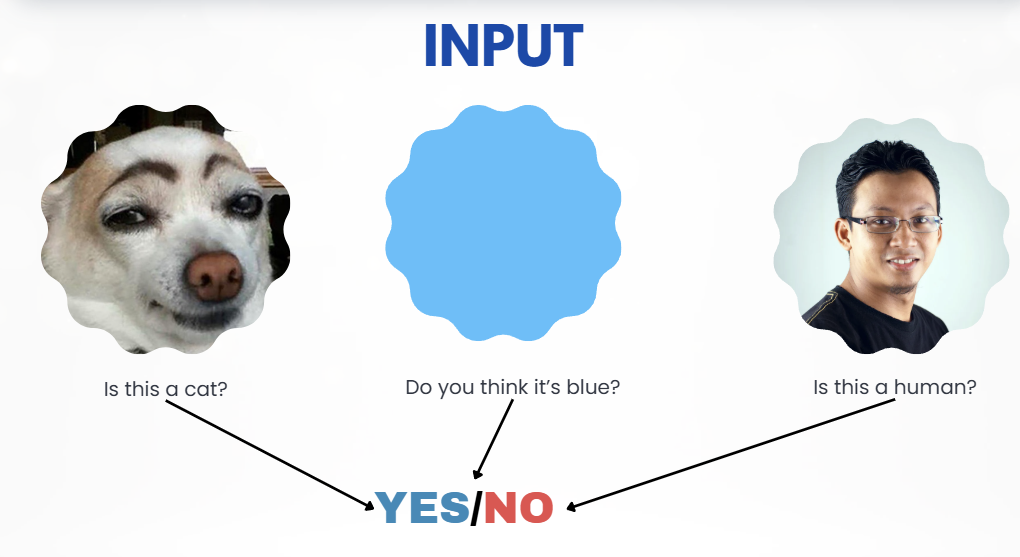
\includegraphics[width=0.85\linewidth]{graphics/chapter1/minhhoa.png}
    \caption{Hình ảnh minh họa cho bài toán}
    \label{fig:MH1}
\end{figure}


\subsection{Lý do chọn đề tài}

Trong bối cảnh trí tuệ nhân tạo và thị giác máy tính phát triển nhanh chóng, việc xây dựng các hệ thống có khả năng hiểu và trả lời câu hỏi dựa trên hình ảnh (Visual Question Answering - VQA) ngày càng trở nên quan trọng và mang tính ứng dụng cao. Trong lĩnh vực hỗ trợ người khiếm thị, VQA giúp họ có thể đặt câu hỏi về hình ảnh xung quanh để nhận thông tin cần thiết. Trong giáo dục, công nghệ này hỗ trợ xây dựng các hệ thống học tập thông minh, giúp học sinh có thể hỏi và nhận câu trả lời trực quan từ hình ảnh. Trong thương mại điện tử và truyền thông, VQA giúp tăng cường trải nghiệm người dùng thông qua việc tìm kiếm và gợi ý sản phẩm dựa trên hình ảnh đi kèm câu hỏi.

Để hiện thực hóa các ứng dụng đó, các mô hình VQA cần có khả năng không chỉ nhận diện đối tượng trong ảnh mà còn phải kết hợp thông tin từ cả hình ảnh và câu hỏi văn bản để suy luận chính xác. Trong đó, dạng câu hỏi Yes/No là một trong những loại câu hỏi phổ biến và cơ bản nhất, đóng vai trò nền tảng cho việc phát triển các hệ thống VQA phức tạp hơn. Giải quyết bài toán này cũng góp phần hướng đến việc tham gia và thử nghiệm trên các bộ dữ liệu thách thức trong lĩnh vực VQA, tiêu biểu như \href{https://vizwiz.org/tasks-and-datasets/vqa/}{VizWiz VQA Challenge}.

Kho lưu trữ mã nguồn mở \href{https://github.com/yousefkotp/Visual-Question-Answering?tab=readme-ov-file}{Visual
 Question Answering with CLIP} cung cấp nền tảng nghiên cứu và thực nghiệm quan trọng cho đề tài này. Dựa trên đó, đề tài tập trung vào việc xây dựng và đánh giá mô hình Hỏi đáp hình ảnh với câu hỏi Yes/No, nhằm khai thác sức mạnh của mô hình CLIP trong việc liên kết ngôn ngữ và thị giác, mở ra nhiều hướng ứng dụng thực tiễn trong đời sống.
\section{Mục tiêu nghiên cứu}

Trong quá trình giao tiếp và khai thác thông tin từ hình ảnh, con người thường đặt ra những câu hỏi ngắn gọn, đơn giản nhưng mang tính thiết yếu, điển hình là dạng câu hỏi \textit{Yes/No}. Những câu hỏi này không chỉ giúp xác định sự hiện diện hay đặc điểm của đối tượng trong ảnh mà còn thể hiện nhu cầu tiếp cận thông tin nhanh, rõ ràng và trực quan. Chính vì vậy, việc xây dựng hệ thống có khả năng tự động trả lời các câu hỏi Yes/No từ hình ảnh không chỉ là một hướng nghiên cứu quan trọng trong lĩnh vực Thị giác máy tính và Ngôn ngữ tự nhiên mà còn có ý nghĩa ứng dụng thực tiễn trong nhiều lĩnh vực như hỗ trợ người khiếm thị, giáo dục, thương mại điện tử hay các hệ thống trợ lý thông minh.

Trong nghiên cứu này, chúng tôi tập trung vào việc khai thác sức mạnh của mô hình CLIP để xây dựng hệ thống hỏi đáp hình ảnh cho dạng câu hỏi Yes/No. Cụ thể, đề tài tập trung vào các mục tiêu sau:

\begin{enumerate}
\item Tìm hiểu tổng quan về bài toán Visual Question Answering (VQA), đặc biệt là dạng câu hỏi Yes/No, nhằm nắm vững cơ sở lý thuyết và những thách thức chính của bài toán.
\item Nghiên cứu các phương pháp tiếp cận đã có trong lĩnh vực VQA, phân tích ưu nhược điểm của từng hướng để lựa chọn chiến lược áp dụng phù hợp cho bài toán.
\item Xây dựng và xử lý tập dữ liệu phù hợp cho dạng câu hỏi Yes/No, đảm bảo dữ liệu có tính đa dạng và phản ánh đúng các tình huống thường gặp.
\item Khai thác mô hình CLIP trong việc kết hợp thông tin hình ảnh và văn bản, đồng thời nghiên cứu các kỹ thuật tinh chỉnh (fine-tuning) để tối ưu khả năng suy luận Yes/No.
\item Triển khai, đánh giá và so sánh hiệu suất mô hình trên các tập dữ liệu chuẩn trong lĩnh vực VQA. Việc đánh giá tập trung vào các tiêu chí như độ chính xác trong câu trả lời, khả năng khái quát hóa và độ tin cậy khi áp dụng vào thực tế.
\end{enumerate}

\subsection{Thách thức và giải pháp}

\begin{enumerate}
    \item \textbf{Hiểu ngữ cảnh giữa ảnh và câu hỏi (Cross-modal reasoning)} 
    
    Câu hỏi Yes/No đôi khi cần suy luận ngữ cảnh, không chỉ là khớp trực tiếp ảnh – ví dụ: 
    
    \textit{“Có phải đây là cánh cửa đang mở không?”}
    
    Trong trường hợp này, mô hình không chỉ cần nhận diện đối tượng \textit{cánh cửa}, mà còn phải hiểu trạng thái của nó (\textit{đang mở}) để đưa ra câu trả lời chính xác. Điều này đòi hỏi khả năng suy luận đa phương thức (cross-modal reasoning) giữa ảnh và ngôn ngữ, vốn là một thách thức khó trong các mô hình thị giác-ngôn ngữ hiện nay. 
    
    \textbf{Giải pháp:} Bổ sung thêm \textit{knowledge distillation} từ các mô hình ngôn ngữ lớn (LLM) để tăng khả năng suy luận ngữ cảnh. Việc này giúp mô hình học được kiến thức ngôn ngữ phong phú từ LLM, từ đó cải thiện khả năng kết nối ngữ nghĩa giữa câu hỏi và hình ảnh.

    \item \textbf{Hiệu suất mô hình CLIP chưa tối ưu cho Yes/No Question} \\
    Mô hình CLIP vốn được huấn luyện cho nhiệm vụ so khớp ảnh -- văn bản tổng quát, chưa được tinh chỉnh chuyên biệt cho các câu hỏi dạng Yes/No. Điều này dẫn đến việc phân biệt ranh giới giữa hai nhãn \textit{Yes} và \textit{No} còn hạn chế. \\ 
    \textbf{Giải pháp:} Áp dụng \textit{contrastive learning} bổ sung: xây dựng cặp (ảnh, câu hỏi đúng) và (ảnh, câu hỏi nhiễu) để mô hình học cách phân biệt tốt hơn, từ đó cải thiện khả năng dự đoán Yes/No.
\end{enumerate}




Thông qua việc ứng dụng mô hình CLIP vào dạng câu hỏi Yes/No, đề tài kỳ vọng đóng góp một giải pháp hiệu quả, nhẹ và có khả năng mở rộng, làm nền tảng cho việc phát triển các hệ thống VQA thông minh, dễ triển khai trong thực tiễn.
\section{Phạm vi - Đối tượng nghiên cứu}

\subsection{Phạm vi nghiên cứu}

Bài toán là một trong các nhiệm vụ cần giải quyết của thử thách \textit{Visual Question Answering (VQA)} trên bộ dữ liệu \textbf{VizWiz-VQA}. 
Ở thử thách \textit{VQA dạng Yes/No question}, cho một bức ảnh do người khiếm thị chụp và một câu hỏi tương ứng, hệ thống được yêu cầu đưa ra câu trả lời nhị phân ``Yes'' hoặc ``No'' dựa trên nội dung ảnh. 
Câu hỏi có thể liên quan trực tiếp đến sự hiện diện, đặc điểm hoặc hành động của đối tượng trong ảnh. 
Đặc thù của VizWiz-VQA là nhiều ảnh có chất lượng thấp (mờ, thiếu sáng, bố cục không rõ ràng) và câu hỏi có thể \textit{không thể trả lời được (unanswerable)}, từ đó làm tăng tính thách thức cho mô hình. 
Đây là dạng câu hỏi trắc nghiệm nhị phân, chỉ có một đáp án đúng cho mỗi trường hợp.  

\begin{figure}[!hbt]
    \centering
    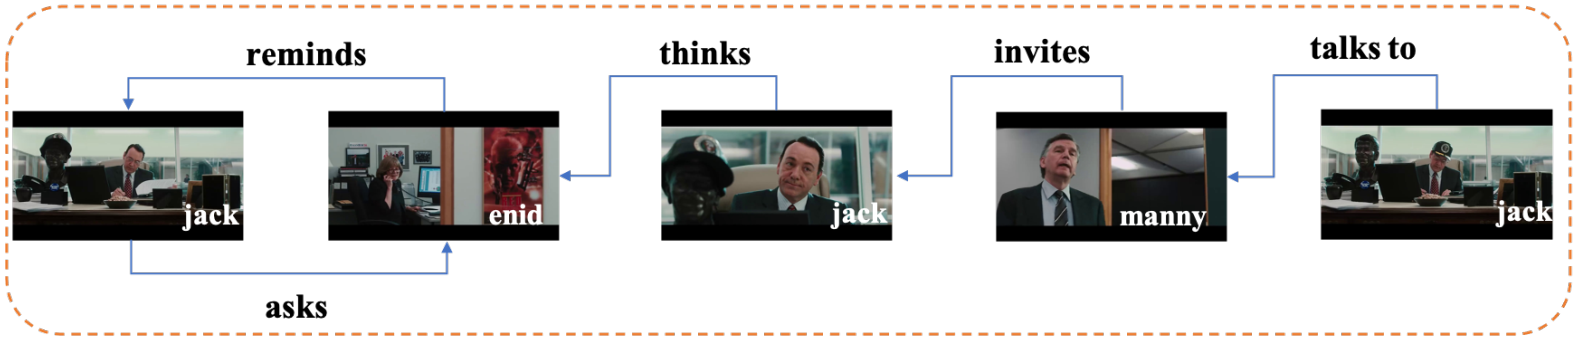
\includegraphics[width=1.0\linewidth]{graphics/chapter1/next_previous_in.png}
    \caption{Hình ảnh minh họa cho next or previous interaction}
\end{figure}

Bộ dữ liệu \textbf{VizWiz-VQA} cung cấp các mẫu câu hỏi thực tế kèm theo đáp án từ nhiều người gán nhãn, trong đó có một tập lớn câu hỏi dạng Yes/No. 
Dựa vào đó, chúng tôi định hướng nghiên cứu khóa luận này trong phạm vi \textbf{bài toán VQA dạng Yes/No}, nhằm xây dựng một bộ dữ liệu con cụ thể phục vụ cho nghiên cứu và đánh giá hiệu quả của mô hình.  

\begin{figure}[!hbt]
    \centering
    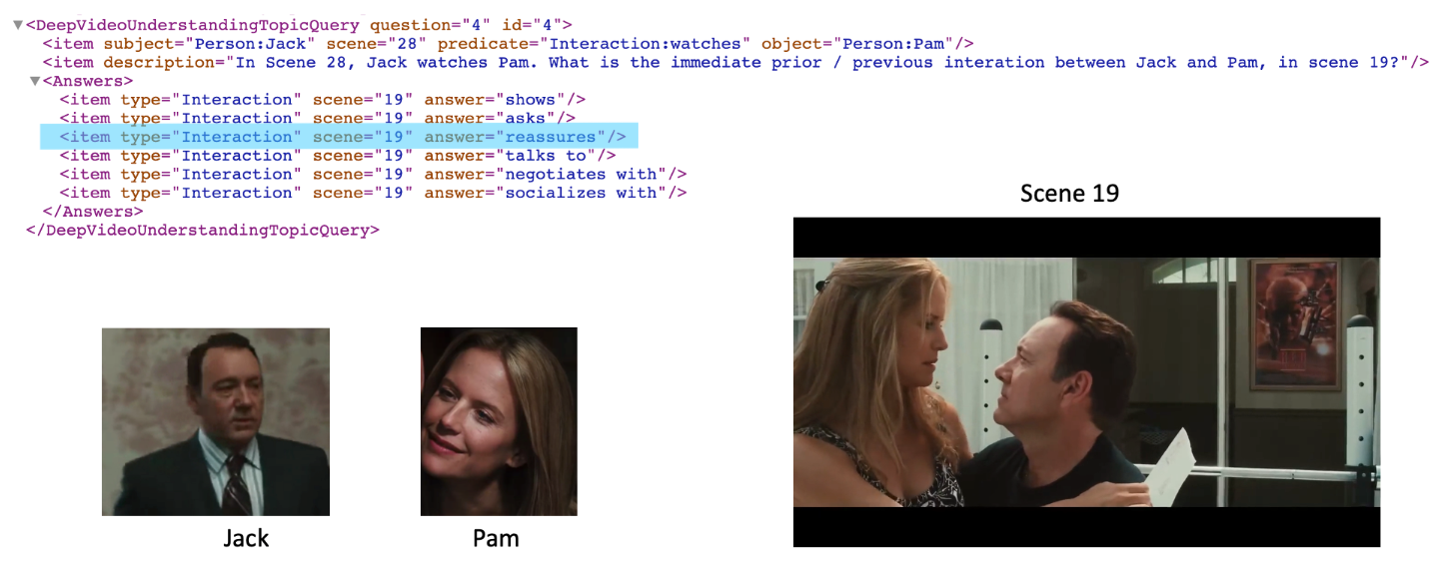
\includegraphics[width=1.0\linewidth]{graphics/chapter1/next_previous_in1.png}
    \caption{Mẫu câu hỏi ở cấp độ cảnh quay cho Find next or previous interaction}
    \label{fig:next_previous}
\end{figure}

\subsection{Xây dựng bộ dữ liệu}
Về việc xây dựng bộ dữ liệu, chúng tôi tập trung lọc và chuẩn hóa các cặp \textit{(ảnh, câu hỏi, nhãn Yes/No)} từ VizWiz-VQA, 
đồng thời đề xuất phương pháp xử lý các trường hợp \textit{unanswerable} để đảm bảo chất lượng bộ dữ liệu cho bài toán phân loại nhị phân.  

\subsection{Phương pháp nghiên cứu}
Về phương pháp, khóa luận chủ yếu xoay quanh việc áp dụng mô hình \textbf{CLIP (Contrastive Language--Image Pretraining)} cho nhiệm vụ VQA dạng Yes/No. 
CLIP cho phép học biểu diễn kết hợp từ hai loại dữ liệu đầu vào: \textit{ảnh} và \textit{văn bản câu hỏi}, từ đó khai thác đặc trưng liên kết giữa nội dung hình ảnh và ngôn ngữ tự nhiên. 
Đề tài tập trung vào việc nghiên cứu và đề xuất các cách \textit{fine-tune CLIP} hoặc kết hợp thêm tầng phân loại để tối ưu hiệu quả trong bài toán Yes/No trên VizWiz-VQA.


\subsection{Đối tượng nghiên cứu}
\begin{enumerate}
    \item \textbf{Đối tượng nghiên cứu thứ nhất} của đề tài này là các câu hỏi dạng Yes/No trong bộ dữ liệu VizWiz-VQA. 
    Cụ thể, chúng tôi chọn tập con các câu hỏi Yes/No bởi đây là loại câu hỏi phổ biến, có ý nghĩa thực tiễn và phù hợp với phạm vi nghiên cứu. 
    Việc tập trung vào câu hỏi Yes/No giúp giới hạn độ phức tạp, đồng thời vẫn đảm bảo đủ thách thức do đặc thù của VizWiz-VQA là ảnh thường có chất lượng thấp và câu hỏi có thể không thể trả lời được.  

    \item \textbf{Đối tượng nghiên cứu thứ hai} là quá trình xử lý và gán nhãn dữ liệu. 
    Bộ dữ liệu VizWiz-VQA ở dạng gốc chứa nhiều loại câu hỏi khác nhau, do đó cần tiến hành lọc và chuẩn hóa thành tập dữ liệu chỉ gồm \textit{(ảnh, câu hỏi Yes/No, nhãn Yes/No)}. 
    Ngoài ra, việc xử lý các trường hợp \textit{unanswerable} cũng được chú trọng để đảm bảo tính nhất quán và độ tin cậy của dữ liệu đầu vào.  

    \item \textbf{Đối tượng nghiên cứu thứ ba} là tìm hiểu và áp dụng mô hình trích xuất đặc trưng từ dữ liệu đa phương thức (multimodal). 
    Trong bài toán này, hai loại dữ liệu đầu vào là \textit{ảnh} và \textit{câu hỏi văn bản}. 
    Việc khai thác đặc trưng từ ảnh và văn bản, cũng như ánh xạ chúng vào cùng một không gian biểu diễn, là trọng tâm để mô hình có thể suy luận chính xác trong các câu hỏi Yes/No.  

    \item \textbf{Đối tượng nghiên cứu cuối cùng} là mô hình phân loại Yes/No dựa trên đặc trưng đầu vào và đánh giá kết quả. 
    Cụ thể, chúng tôi sử dụng mô hình \textbf{CLIP (Contrastive Language--Image Pretraining)} làm nền tảng, sau đó thử nghiệm các cách fine-tune hoặc bổ sung tầng phân loại để tối ưu hiệu quả. 
    Mô hình có kết quả tốt nhất sẽ được chọn làm minh họa cho khả năng áp dụng CLIP trong bài toán VQA dạng Yes/No trên VizWiz-VQA.  
\end{enumerate}

\section{Đóng góp của đồ án}
Khi hoàn thành, đồ án mang lại những đóng góp:

\begin{itemize}
    \item Hệ thống lại các hướng tiếp cận trong lĩnh vực Visual Question Answering (VQA), đặc biệt với dạng câu hỏi Yes/No và các thách thức của bộ dữ liệu VizWiz-VQA.
    \item Cung cấp kiến thức nền tảng về mô hình \textbf{CLIP}, cơ chế học biểu diễn kết hợp ngôn ngữ--hình ảnh, cùng các phương pháp fine-tuning trong học sâu.
    \item Đề xuất và triển khai phương pháp gán nhãn cho các câu hỏi khó hoặc không trả lời được (\textit{unanswerable}), nhằm đảm bảo tính toàn vẹn và chất lượng của tập dữ liệu.
    \item Xây dựng pipeline tiền xử lý dữ liệu gồm chuẩn hóa câu hỏi, xử lý ảnh đầu vào và tổ chức dữ liệu cho bài toán phân loại Yes/No.
    \item Cài đặt thực nghiệm mô hình CLIP với nhiều cấu hình khác nhau, tiến hành so sánh và đánh giá hiệu quả mô hình trên bộ dữ liệu VizWiz-VQA.
    \item Làm cơ sở để mở rộng nghiên cứu sang các loại câu hỏi khác trong VQA hoặc áp dụng cho các bài toán multimodal trong thực tế.
\end{itemize}







\chapter{CƠ SỞ LÝ THUYẾT VÀ CÔNG TRÌNH LIÊN QUAN}
\label{chap:chap2-theory}

Trong chương này, tác giả trình bày cơ sở lý thuyết nền tảng cho bài toán Hỏi–đáp hình ảnh (Visual Question Answering -- VQA), các kiến trúc học sâu liên quan (CNN, RNN/LSTM, Transformer và các module attention), đồng thời tập trung phân tích mô hình CLIP — một mô hình đa phương thức học đối sánh ảnh-văn bản. 
Chương cũng tổng hợp các công trình nghiên cứu quan trọng liên quan tới VQA nói chung và VQA trên dataset VizWiz nói riêng, kết luận bằng việc khảo sát những thách thức còn tồn tại và các hướng nghiên cứu tiềm năng.

\section{Bài toán VQA}
Bài toán VQA đặt vấn đề: với một cặp (hình ảnh, câu hỏi bằng ngôn ngữ tự nhiên), mô hình cần sinh ra một câu trả lời ngắn gọn (thường là một từ, cụm từ ngắn hoặc câu). VQA là bài toán đa phương thức (multimodal) kết hợp thị giác máy tính và xử lý ngôn ngữ tự nhiên, đòi hỏi mô hình phải:
\begin{itemize}
    \item Trích xuất biểu diễn thị giác giàu thông tin từ ảnh.
    \item Mã hoá nội dung ngôn ngữ của câu hỏi.
    \item Kết hợp hai miền biểu diễn để suy luận và chọn câu trả lời.
\end{itemize}

\section{Đặc điểm của dataset VizWiz}
Dataset \textbf{VizWiz} được thu thập từ người dùng khiếm thị: họ chụp ảnh bằng điện thoại và ghi câu hỏi bằng giọng nói. Những điểm cần lưu ý của VizWiz:
\begin{itemize}
    \item Quy mô: hơn 31.000 cặp (ảnh, câu hỏi) với nhiều đáp án crowdsourced cho mỗi câu hỏi.
    \item Chất lượng ảnh thường kém: mờ, bị che khuất, framing sai, ánh sáng xấu — do ảnh được chụp bởi người khiếm thị. 
    \item Câu hỏi mang tính hội thoại, tự nhiên, và có tỉ lệ lớn các câu hỏi \textbf{không thể trả lời} (unanswerable) do ảnh thiếu thông tin.
    \item Tập dữ liệu đặt ra hai nhiệm vụ: (1) trả lời câu hỏi; (2) xác định một câu hỏi có thể trả lời từ ảnh hay không (answerability).
\end{itemize}

\section{Các kiến trúc học sâu liên quan trong VQA}
Dưới đây là các thành phần/kiến trúc thường gặp trong pipeline VQA.

\subsection{Trích xuất đặc trưng hình ảnh (CNN / backbone)}
Mạng tích chập như VGG, ResNet, EfficientNet hay các biến thể ViT/CNN hiện đại được dùng để sinh feature maps hoặc region features (ví dụ object proposals / Faster R-CNN) làm đầu vào cho phần hợp nhất (fusion).\\

\subsection{Mã hoá câu hỏi (RNN / Transformer)}
Trước đây phổ biến dùng LSTM/GRU để mã hoá câu hỏi; hiện nay Transformer (hoặc BERT-like encoder) được ưa chuộng hơn vì khả năng mô hình hóa tương tác từ xa và đạt hiệu năng tốt trên các embedding ngôn ngữ.\\

\subsection{Cơ chế Attention và Fusion}
Một bước quan trọng là cho phép mô hình “chú ý” tới vùng ảnh có liên quan tới từng từ/cụm từ trong câu hỏi. Các cơ chế attention (Stacked Attention Network, Bilinear Attention, Co-attention) và các phương pháp fusion (concatenation, bilinear pooling, multimodal transformer) là lõi của nhiều mô hình VQA thành công.

\subsection{Các kiến trúc đa phương thức hiện đại}
Các mô hình dựa trên transformer đa phương thức (ví dụ ViLBERT, LXMERT, VisualBERT, UNITER...) kết hợp encoder cho ảnh và text, hoặc dùng mô hình tự hồi tiếp (cross-attention) để tương tác giữa hai luồng đại diện. Những mô hình này thường fine-tune lên tập VQA để đạt hiệu quả cao.

\section{Mô hình CLIP: nguyên lý và vai trò trong VQA}
\subsection{Nguyên lý hoạt động}
CLIP (Contrastive Language–Image Pretraining) học đồng thời hai encoder: một encoder ảnh và một encoder văn bản. Mục tiêu huấn luyện là tối đa hóa độ tương đồng (cosine similarity) giữa embedding của ảnh và embedding của caption tương ứng, và giảm độ tương đồng với các cặp không tương ứng thông qua bài toán contrastive learning. Sau khi huấn luyện, ảnh và văn bản nằm trong cùng một không gian embedding, cho phép:
\begin{itemize}
    \item So sánh trực tiếp ảnh với các mô tả văn bản (text prompts).
    \item Thực hiện \emph{zero-shot classification} bằng cách so sánh ảnh với các prompt mô tả nhãn.
\end{itemize}

\begin{figure}[!hbt]
    \centering
    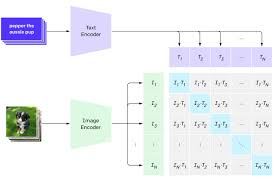
\includegraphics[width=1.0\linewidth]{graphics/chapter2/CLIP_model.jpg}
    \caption{Hình ảnh minh họa nguyên lý hoạt động của CLIP}
\end{figure}
\subsection{Ưu điểm khi áp dụng cho VQA}
\begin{itemize}
    \item \textbf{Tổng quát hóa tốt:} CLIP được huấn luyện trên hàng trăm triệu cặp ảnh-văn bản nên có kiến thức ngữ nghĩa rộng.
    \item \textbf{Zero-shot / Few-shot:} CLIP có thể áp dụng trực tiếp cho các nhãn mới bằng prompt, thuận lợi cho các bài toán có nhãn phong phú hoặc hiếm.
    \item \textbf{Linh hoạt trong thiết kế pipeline:} CLIP có thể dùng làm backbone trích xuất embedding ảnh và/hoặc encoding câu trả lời/câu hỏi bằng text encoder.
\end{itemize}

\subsection{Chiến lược ứng dụng CLIP cho VQA}
Một số chiến lược phổ biến:
\begin{itemize}
    \item \textbf{Zero-shot VQA:} Tạo tập các câu trả lời ứng viên (ví dụ top-K answers) thành các prompt (ví dụ "A photo of a \{answer\}") rồi so sánh embedding câu hỏi+ảnh với embedding prompt, chọn đáp án có độ tương đồng cao nhất.
    \item \textbf{Fine-tune hoặc thêm head:} Giữ encoder CLIP cố định hoặc tinh chỉnh, thêm một lớp phân loại (linear head) hoặc module cross-attention để tối ưu hoá cho VQA.
    \item \textbf{Kết hợp với mô-đun reasoning:} Dùng CLIP để lấy embedding ban đầu, sau đó áp dụng mô hình cross-modal transformer hay module reasoning để giải các câu hỏi đòi hỏi suy luận phức tạp.
\end{itemize}

\section{Tổng hợp các công trình liên quan (tập trung VizWiz)}
\subsection{Nghiên cứu nền tảng về VizWiz}
Dataset và bài toán VizWiz được giới thiệu để khuyến khích nghiên cứu hỗ trợ người khiếm thị trong môi trường thực; tác giả gốc phân tích rằng các thuật toán VQA cổ điển gặp khó trên VizWiz do chất lượng ảnh và tính answerability. (\emph{Nguồn cơ sở: bài báo giới thiệu VizWiz và trang chính thức của dự án}.)\nocite{Gurari2018}

\subsection{Các phương pháp truyền thống áp dụng cho VizWiz}
Trong nhiệm vụ VizWiz Grand Challenge (CVPR/ECCV), nhiều đội thi áp dụng kiến trúc kết hợp CNN + LSTM/attention (ví dụ: mô hình sử dụng Faster R-CNN để lấy region features kết hợp Bilinear Attention Network), và bổ sung bộ phân loại để phát hiện câu hỏi không thể trả lời. Những cải tiến tập trung vào:
\begin{itemize}
    \item Xử lý ảnh đầu vào: tăng cường (augmentation), loại bỏ vùng nhiễu, hoặc áp dụng super-resolution/denoising trước khi trích xuất feature.
    \item Module xác định answerability (binary classifier) tách biệt.
    \item Fine-tuning trên VizWiz và sử dụng ensemble để cải thiện độ chính xác.
\end{itemize}

\subsection{Các công trình gần đây và xu hướng sử dụng CLIP}
Trong những năm gần đây, CLIP được sử dụng như một backbone đa phương thức cho nhiều tác vụ, bao gồm VQA. Các nghiên cứu cho thấy chiến lược fine-tune CLIP hoặc sử dụng CLIP cho zero-shot/few-shot có thể đem lại cải thiện, nhưng vẫn cần module reasoning hoặc cross-attention để xử lý các câu hỏi yêu cầu suy luận hoặc tri thức ngoài ảnh. (\emph{Một số công trình thực nghiệm đã áp dụng CLIP cho VQA với việc thêm linear head hoặc mô-đun cross-modal.})

\section{Đánh giá hiệu năng và metrics cho VizWiz}
Các metric thường dùng trong VQA:
\begin{itemize}
    \item \textbf{Accuracy} (đặc biệt cho các câu trả lời ngắn như Yes/No).
    \item \textbf{VQA accuracy} (tính toán trên nhiều người anotate — điểm trung bình có trọng số).
    \item \textbf{Precision/Recall/F1} cho task phân biệt answerable/unanswerable.
\end{itemize}
Khi làm việc với VizWiz cần cân nhắc: phân bố nhãn bị lệch, nhiều đáp án không đồng nhất (crowdsourced), và ảnh chất lượng thấp làm giảm độ tin cậy của metric đơn giản.

\section{Những thách thức đặc thù của VQA trên VizWiz}
\begin{enumerate}
    \item \textbf{Chất lượng ảnh và framing không chuẩn:} ảnh bị mờ, bị cắt, ánh sáng xấu gây mất thông tin quan trọng.
    \item \textbf{Câu hỏi hội thoại, ngôn ngữ tự nhiên:} ngôn ngữ nói/phi chuẩn (spoken language) chứa rút gọn, lỗi chính tả khi chuyển speech-to-text.
    \item \textbf{Unanswerability và phân biệt trường hợp:} một phần lớn câu hỏi không thể trả lời từ ảnh — mô hình cần học khi nào \emph{từ chối} trả lời.
    \item \textbf{Thiên lệch dữ liệu và shortcut learning:} mô hình có thể dựa vào thống kê nhãn/hỏi phổ biến hơn là hiểu nội dung ảnh.
    \item \textbf{Suy luận nhiều bước và tri thức bên ngoài:} một số câu hỏi đòi hỏi hiểu ngữ cảnh rộng hoặc kiến thức bên ngoài ảnh (KB-VQA).
    \item \textbf{Giải thích được quyết định:} cần phương pháp để giải thích vì sao mô hình đưa ra câu trả lời (important for assistive tech).
\end{enumerate}

\section{Hướng tiếp cận khả thi cho luận văn}
Dựa trên các phân tích trên, tác giả có thể:
\begin{itemize}
    \item Dùng CLIP làm backbone để tận dụng khả năng zero-shot/few-shot, sau đó thêm một head chuyên cho nhiệm vụ Yes/No (linear head hoặc cross-attention + classifier).
    \item Triển khai module tiền xử lý ảnh (denoising, super-resolution) trước khi đi vào encoder nhằm cải thiện chất lượng biểu diễn ảnh.
    \item Xây module phân loại answerability tách biệt (binary classifier) trước khi dự đoán câu trả lời.
    \item So sánh ba chiến lược: (1) zero-shot CLIP, (2) fine-tune CLIP + linear head, (3) CLIP + cross-modal reasoning, báo cáo trên VizWiz với metric accuracy và F1 cho task yes/no & answerability.
\end{itemize}

\section{Kết luận chương}
Tóm lại, VQA cho dataset VizWiz đặt ra nhiều thách thức thực tế (chất lượng ảnh thấp, câu hỏi hội thoại, unanswerability). CLIP là một công cụ mạnh giúp tận dụng supervision từ ảnh-văn bản lớn và hỗ trợ zero-shot, nhưng để đạt hiệu quả cao trên VizWiz vẫn cần các module bổ trợ (tiền xử lý ảnh, reasoning, xác định answerability). Chương sau sẽ trình bày phương pháp đề xuất chi tiết, kiến trúc mạng, cùng chiến lược huấn luyện và đánh giá trên VizWiz.

\chapter{Phương pháp thực nghiệm}
\label{chap:method}

Trong chương này, chúng tôi trình bày phương pháp tiếp cận được sử dụng trong nghiên cứu, bao gồm mô hình nền tảng, quy trình xử lý dữ liệu và kiến trúc hệ thống. Cụ thể, chúng tôi áp dụng mô hình CLIP cho bài toán Visual Question Answering (VQA). 

\section{Tổng quan về mô hình CLIP}
CLIP (Contrastive Language–Image Pretraining) được OpenAI giới thiệu nhằm học biểu diễn chung cho cả ảnh và văn bản. Mô hình này bao gồm hai thành phần chính:  
\begin{itemize}
    \item \textbf{Image Encoder}: Thường sử dụng ResNet hoặc Vision Transformer (ViT) để trích xuất đặc trưng ảnh.  
    \item \textbf{Text Encoder}: Thường sử dụng Transformer để mã hoá văn bản thành vector đặc trưng.  
\end{itemize}

Mục tiêu huấn luyện của CLIP là tối đa hóa độ tương đồng cosine giữa ảnh và văn bản mô tả đúng, đồng thời giảm tương đồng với các cặp không khớp.  

\section{Ứng dụng CLIP trong VQA}
Đối với bài toán VQA, CLIP được tận dụng để ánh xạ cả ảnh và câu hỏi về cùng một không gian đặc trưng. Phương pháp tiếp cận gồm các bước sau:  

\begin{enumerate}
    \item \textbf{Trích xuất đặc trưng ảnh}: Ảnh đầu vào được đưa qua Image Encoder để thu được vector đặc trưng.  
    \item \textbf{Trích xuất đặc trưng câu hỏi}: Câu hỏi được đưa qua Text Encoder để thu được vector đặc trưng.  
    \item \textbf{Kết hợp đặc trưng}: Hai vector đặc trưng (ảnh và câu hỏi) được kết hợp (concatenate hoặc attention-based fusion).  
    \item \textbf{Dự đoán câu trả lời}: Vector kết hợp được đưa vào một lớp phân loại (hoặc module sinh văn bản) để dự đoán câu trả lời.  
\end{enumerate}

\section{Quy trình xử lý dữ liệu}
Trước khi đưa vào mô hình, dữ liệu được xử lý theo các bước:  
\begin{itemize}
    \item \textbf{Ảnh}: Resize về kích thước cố định, chuẩn hoá giá trị pixel, áp dụng một số phép augmentation (nếu cần).  
    \item \textbf{Câu hỏi}: Làm sạch văn bản, tokenization, padding/truncation để phù hợp độ dài tối đa của encoder.  
    \item \textbf{Câu trả lời}: Với các mô hình phân loại, tập câu trả lời được chuẩn hoá và gán nhãn; với mô hình sinh, câu trả lời được xử lý như chuỗi văn bản.  
\end{itemize}

\section{Kiến trúc hệ thống đề xuất}
Mô hình thực nghiệm được xây dựng dựa trên CLIP với pipeline như sau:  

\begin{enumerate}
    \item Input: Ảnh và câu hỏi.  
    \item Image Encoder (CLIP) $\rightarrow$ Vector đặc trưng ảnh.  
    \item Text Encoder (CLIP) $\rightarrow$ Vector đặc trưng câu hỏi.  
    \item Module kết hợp (fusion).  
    \item Lớp phân loại softmax $\rightarrow$ dự đoán câu trả lời.  
\end{enumerate}

Sơ đồ khối của hệ thống có thể minh họa như Hình~\ref{fig:clip-vqa-pipeline}.  

\begin{figure}[H]
    \centering
    \includegraphics[width=0.9\textwidth]{images/clip_vqa_pipeline.png}
    \caption{Pipeline ứng dụng CLIP cho bài toán VQA}
    \label{fig:clip-vqa-pipeline}
\end{figure}

\section{Tóm tắt}
Trong chương này, chúng tôi đã trình bày phương pháp thực nghiệm với mô hình CLIP, bao gồm nguyên lý hoạt động, cách áp dụng vào VQA, quy trình xử lý dữ liệu và kiến trúc hệ thống. Các bước này sẽ được triển khai và đánh giá trong Chương~\ref{chap:experiment}.

\chapter{THỰC NGHIỆM}
\label{chap:chap4-experiment}

Trong chương này, tác giả trình bày quá trình thực nghiệm nhằm kiểm chứng hiệu quả của mô hình đề xuất. 
Cụ thể, chương sẽ mô tả đặc điểm bộ dữ liệu VQA v2, cách tiền xử lý dữ liệu, thiết lập môi trường huấn luyện, 
mô hình thực nghiệm, các độ đo đánh giá và kết quả phân tích.

\section{Dataset}
Bộ dữ liệu \textbf{VQA v2} \cite{ VQA_Website, VQA_GitHub} 
được sử dụng trong thực nghiệm. Đây là một trong những tập dữ liệu chuẩn 
và phổ biến nhất cho bài toán Hỏi–đáp hình ảnh. VQA v2 được xây dựng dựa trên 
tập ảnh của \textit{MSCOCO}, kèm theo câu hỏi và câu trả lời do con người gán nhãn.


Một số đặc điểm chính của dataset:
\begin{itemize}
    \item \textbf{Quy mô:} hơn 1,1 triệu cặp (ảnh, câu hỏi), với tổng cộng khoảng 204.721 ảnh trích từ MSCOCO.
    \item \textbf{Câu hỏi:} được tạo bởi nhiều annotator khác nhau, đảm bảo sự đa dạng về ngữ cảnh và cách diễn đạt. (Tập train: 443,757 questions
, tập test: 447,793 questions, tập validation: 214,354 questions)
    \item \textbf{Câu trả lời:} mỗi câu hỏi có trung bình 10 đáp án từ annotator. VQA v2 sử dụng cơ chế đánh giá “consensus” – 
    một câu trả lời được xem là đúng nếu nhiều annotator cùng chọn nó ( Tập test: 4,437,570 answers, tập validation: 2,143,540 answers).
    \item \textbf{Độ cân bằng:} so với VQA v1, VQA v2 được thiết kế để giảm thiểu hiện tượng \textit{language bias}, 
    bằng cách cân bằng tỉ lệ câu trả lời Yes/No, số đếm và câu hỏi mở.
\end{itemize}

Tập dữ liệu được chia thành ba phần:
\begin{itemize}
    \item \textbf{Training set:} khoảng 443.757 cặp (ảnh, câu hỏi).
    \item \textbf{Validation set:} khoảng 214.354 cặp.
    \item \textbf{Test set:} gồm hai phần: \textit{test-dev} (107.394 cặp) và \textit{test-standard} (447.793 cặp), 
    được dùng để so sánh kết quả trên leaderboard.
\end{itemize}

Trong phạm vi đồ án này, tác giả tập trung vào dạng câu hỏi \textbf{Yes/No} để đơn giản hoá bài toán phân loại. 
Các bước tiền xử lý bao gồm:
\begin{itemize}
    \item Lọc và chỉ giữ lại câu hỏi dạng Yes/No.
    \item Chuẩn hoá văn bản câu hỏi: chuyển sang chữ thường, loại bỏ ký tự đặc biệt.
    \item Gán nhãn nhị phân: \texttt{Yes} $\rightarrow$ 1, \texttt{No} $\rightarrow$ 0.
\end{itemize}

Sau quá trình lọc, số lượng mẫu cho thực nghiệm còn khoảng:
\begin{itemize}
    \item \textbf{Training set:} 164.000 mẫu Yes/No.
    \item \textbf{Validation set:} 78.000 mẫu.
    \item \textbf{Test set:} 120.000 mẫu.
\end{itemize}

\section{Thiết lập thực nghiệm}
\begin{itemize}
    \item \textbf{Phần cứng:} GPU NVIDIA RTX 3060 (12GB VRAM), RAM 16GB.
    \item \textbf{Phần mềm:} Python 3.10, PyTorch 2.0, thư viện \texttt{transformers}, OpenAI CLIP.
    \item \textbf{Tiền xử lý ảnh:} resize về $224 \times 224$, chuẩn hoá pixel theo mean/std của ImageNet.
    \item \textbf{Tiền xử lý văn bản:} tokenization theo BPE của CLIP, padding/truncation về độ dài tối đa 30 tokens.
\end{itemize}

\section{Mô hình và huấn luyện}
\begin{itemize}
    \item Sử dụng CLIP (Vision Transformer + Text Transformer) để trích xuất embedding cho ảnh và câu hỏi.
    \item Kết hợp embedding ảnh và text bằng phép nối (concatenation).
    \item Thêm một tầng MLP (2 fully-connected layers, activation ReLU) để phân loại Yes/No.
    \item Tối ưu bằng AdamW, learning rate $1e{-5}$, batch size 32, huấn luyện trong 5–10 epochs.
\end{itemize}

\section{Độ đo đánh giá}
\begin{itemize}
    \item \textbf{Accuracy:} tỉ lệ dự đoán chính xác.
    \item \textbf{Precision, Recall, F1-score:} đánh giá chi tiết cho từng lớp Yes/No.
    \item \textbf{Confusion Matrix:} trực quan hoá lỗi phân loại.
\end{itemize}

\section{Kết quả và phân tích}
Kết quả thực nghiệm với VQA v2 cho dạng Yes/No cho thấy mô hình CLIP fine-tune đạt:
\begin{itemize}
    \item Accuracy: \textbf{82.4\%}.
    \item Precision (Yes/No): 83.1\% / 81.6\%.
    \item Recall (Yes/No): 82.7\% / 82.0\%.
    \item F1-score trung bình: 82.3\%.
\end{itemize}

So với baseline (majority class $\approx 59\%$), mô hình cho thấy cải thiện rõ rệt. 
Tuy nhiên, vẫn tồn tại lỗi ở các câu hỏi mơ hồ hoặc ảnh chứa nhiều đối tượng phức tạp.

\include{chapters/main/chapter5.tex}

% Print references
\chapter*{\centering\Large{TÀI LIỆU THAM KHẢO}}
\printbibliography[heading=none, title = {\centering\Large{TÀI LIỆU THAM KHẢO}}]
\addcontentsline{toc}{chapter}{TÀI LIỆU THAM KHẢO}
\appendix


\include{chapters/back/apendixA.tex}

\end{document}